\chapter{INTRODUÇÃO}
\label{chap:contextualizacao}

Todo TCC começa com uma Introdução, aquela seção onde você tenta convencer o leitor de que o seu tema é relevante e indispensável para a humanidade - mesmo que seja só um sistema que manda notificação quando a pizza sai do forno.

A introdução também serve para contar uma história emocionante: do problema que ninguém resolvia, até a sua solução (que surgiu às 3h da manhã, enquanto você rolava na cama tentando dormir).

Você descreve o contexto, apresenta o desafio, dramatiza um pouco e termina com uma pergunta do tipo: \enquote{Diante disso, como garantir a eficiência da metodologia proposta em cenários reais?} Você não faz ideia. O seu trabalho é justamente encontrar a resposta.

Exemplo de como incluir uma ilustração: primeiro, explique e dê o contexto da ilustração, e a referencie, gráfico \ref{graph:anos_trabalhos_selecionados_v2}.

%você pode organizar melhor suas imagens se criar subpastas nos chapters
\begin{grafico}[ht!]
\centering

\caption{\textmd{Exemplo de gráfico.}}
\label{graph:anos_trabalhos_selecionados_v2}
\fcolorbox{gray}{white}{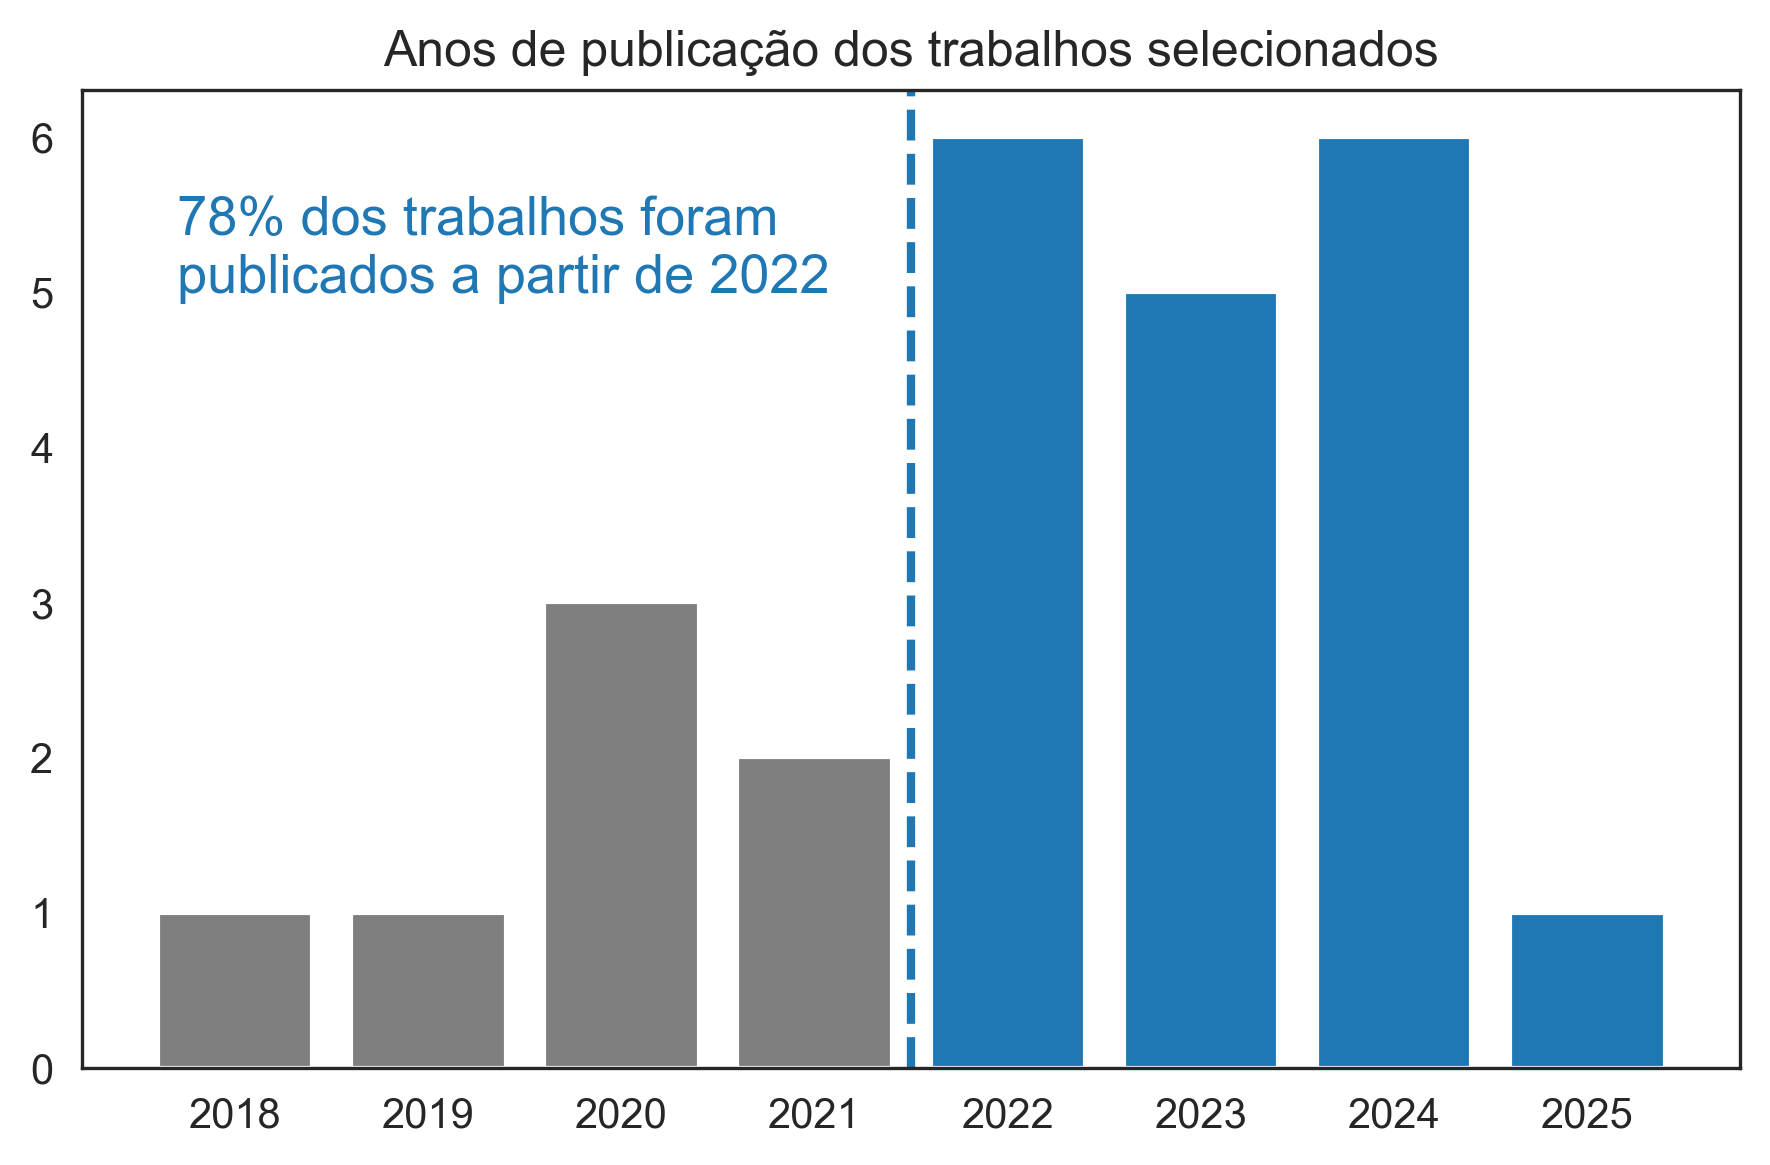
\includegraphics[width=0.9\textwidth]{images/resultados/anos_trabalhos_selecionados_v2.png}}

\fonteref{Elaborado pelo autor.}
\end{grafico}

Mais uma vez, cite o contexto: "Bla bla bla bla" figura \ref{fig:figura_panda}.

%você pode organizar melhor suas imagens se criar subpastas nos chapters
\begin{figure}[ht!]
\centering

\caption{\textmd{Exemplo de figura.}}
\label{fig:figura_panda}
\fcolorbox{gray}{white}{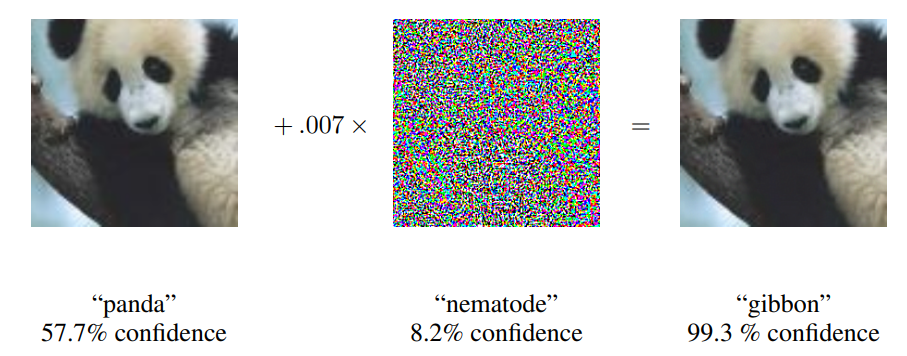
\includegraphics[width=0.9\textwidth]{images/resultados/figura_panda.png}}

\fonteref{Elaborado pelo autor.}
\end{figure}


Bla bla bla bla diagrama \ref{diag:fluxo_addon}

%você pode organizar melhor suas imagens se criar subpastas nos chapters
\begin{diagrama}[ht!]
\centering

\caption{\textmd{Exemplo de fluxograma.}}
\label{diag:fluxo_addon}
\fcolorbox{gray}{white}{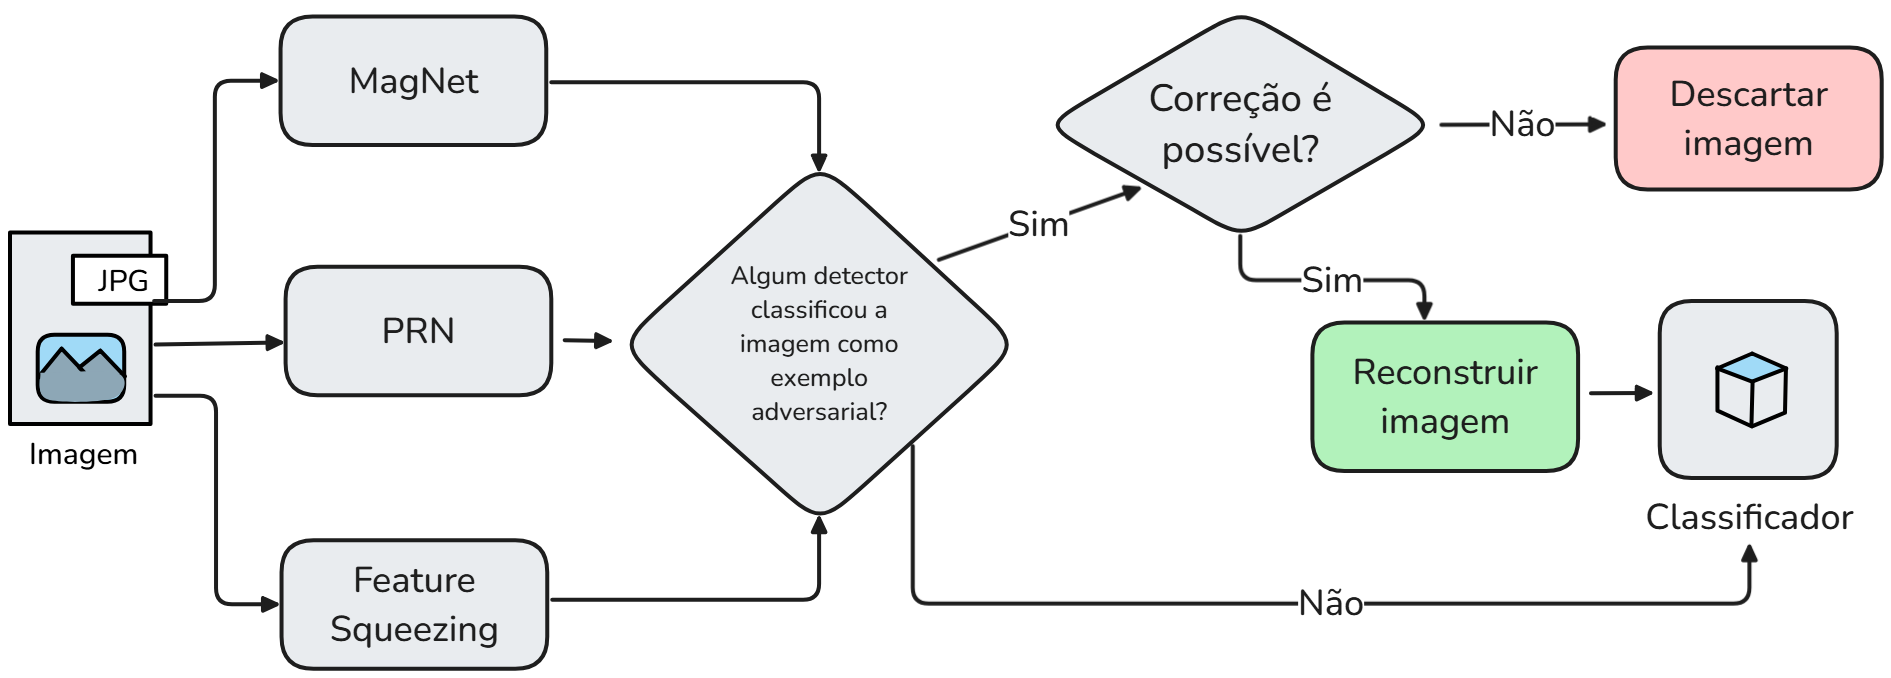
\includegraphics[width=0.9\textwidth]{images/resultados/fluxo_addon.png}}

\fonteref{Elaborado pelo autor.}
\end{diagrama}

Por fim, não se esqueça de incluir a pergunta norteadora: \textit{\enquote{Como otimizar o processo de aquecimento de pizza utilizando softwares com sistemas de notificação?}} Ou melhor: Será que se eu juntar esses negócio aqui, vai dar bom?
